\documentclass[a4paper,12pt,oneside]{book} % A4 a pagina singola 12pt font
\linespread{1.5} % interlinea
\usepackage{geometry}
\geometry{top=2cm,bottom=2cm,left=3.5cm,right=3.5cm} % Impostiamo il valore dei margini.
\usepackage[utf8]{inputenc}
\usepackage{tikz,pgf}
\usepackage{amsfonts}
\usepackage[italian]{babel} %% Abbiamo istruito LaTeX ad usare la lingua italiana.
\usepackage{todonotes}
\usepackage{subfig}
\usepackage{fancyhdr}
\setlength{\parindent}{0cm}

\usepackage[
backend=biber,
style=numeric,
sorting=none
]{biblatex}
\addbibresource{bibliografia.bib}


%TEOREMI E DEFINIZIONI:
\usepackage{amsmath} %per teoremi ecc
\usepackage{amsthm} %per le definizioni
\newtheorem{theorem}{Teorema}
\newtheorem{lemma}{Lemma}
\newtheorem{definition}{Definizione}
\newtheorem{notion}{Nozione}
\newtheorem{conjecture}{Congettura}
\newtheorem{nb}{Nota Bene}
\newtheorem{ex}{Esempio}

%Fare un comando per gli esempi

%NOTE A PIE' DI PAGINA:
\newcounter{myfootnote}
\setcounter{myfootnote}{1}

\newcommand{\myfootnote}[1]{%
    \textsuperscript{\arabic{myfootnote}}%
    \footnotetext[\arabic{myfootnote}]{#1}%
    \stepcounter{myfootnote}%
}

%SCHEMI DA LIBRO
%\usepackage{booktabs} % Per le linee più spesse
\usepackage{array} %per rappresentare gli array

\usepackage{graphicx}
\usepackage{float}
\usepackage{csquotes}
\usepackage{amsmath}
\usepackage{numprint}
\usepackage{pgfplots}
\usepackage{pgfplotstable}
\usepackage{tocbibind}
\setcounter{tocdepth}{3}
\usepackage{hyperref}

\usepackage{fancyhdr}
\pagestyle{fancy}
\renewcommand{\headrulewidth}{0pt}
\fancyhf{}
\fancyhead[L]{}
\fancyfoot[C]{\thepage}

\graphicspath{{imgs/}} %% cartella dalla quale ricavare le immagini %%

\setlength {\marginparwidth }{2cm} 
\pgfplotsset{compat=1.16}

\newenvironment{dedication}
  {\clearpage           % we want a new page
   \thispagestyle{empty}% no header and footer
   \vspace*{\stretch{1}}% some space at the top 
   \itshape             % the text is in italics
   \raggedleft          % flush to the right margin
  }
   {\par % end the paragraph
   \vspace{\stretch{3}} % space at bottom is three times that at the top
   \clearpage           % finish off the page
  }
  
\begin{document}
%% Frontespizio %%
\begin{titlepage}
    \begin{center}
    \vspace*{0.2cm}
    \begin{figure}[H]
        \centering
        %%\includegraphics[width=0.8\textwidth]{imgs/logo.png}
    \end{figure}
        \vspace{5mm}
%% Dipartimento %%
    	\uppercase{\normalsize Dipartimento di Ingegneria Informatica, Modellistica, Elettronica e Sistemistica}\\
    \end{center}
    \begin{center}
%% Corso di Laurea %%
    	\large{ Corso di Laurea Triennale in Ingegneria Informatica}\\
        \vspace{3mm}
        \large{\bf Tesi di Laurea}\\
    	\vspace{10mm}
%% Titolo della Tesi %%
    {\LARGE{\bf Crittografia quantistica e cyber security}}\\	
     \vspace{7mm}
    \end{center}
    
    \vspace{25mm}
    \noindent
    \begin{minipage}[t]{0.47\textwidth}
%% Relatore %%
    	{\large{ Relatore:\vspace*{0.22cm}\\\bf Prof. \\Floriano De Rango}}
    	\vspace{12mm}
    \end{minipage}
    \hfill
    \begin{minipage}[t]{0.4\textwidth}\raggedleft
%% Candidato %%
    	{\large{Candidato: \\ \bf Giovanni Lorenzo Murfuni\\ Mat. 230599}}
    \end{minipage}
    
    \vspace{30mm}
    
%% Anno Accademico %%
    \centering{\large \uppercase{ Anno Accademico 23/24}}

\end{titlepage}

\begin{dedication}
Dedica e Ringraziamenti...
\end{dedication}

%% Corpo della tesi %%

%%\chapter*{Sommario} %% In questa zona inseriamo l'abstract del nostro documento. %%
%%Inserisci abstract: ...


\tableofcontents
\chapter{Introduzione}
\section{Come funziona l'esame?}
Il professore prende le presenze e assegnerà dei progettini, solo con presenze e progrttini, si arriva al 18.
L'esame consiste in un esercizio, una domanda teorica e poi un orale.

\section{Concetti Iniziali}
\begin{definition}
    La matematica del continuo si basa sul concetto di numero reale ed è ampiamente usata nelle scienze applicate. 
\end{definition}
\begin{definition}
    Il calcolo numerico è una branca della matematica che si occupa dello sviluppo di algoritmi per la risoluzione 
    dei problemi alla matematica del continuo.
\end{definition}
Di base, il calcolo numerico si occupa i problemi di risoluzione prettamente numerici e dei problemi di 
approssimazione.

\subsection{Problemi della matematica del continuo}
I problemi classici nella matematica del continuo sono come:
\textbf{La risoluzione di funzioni} come $\mathit{f}(x) = 0$, dove $x \in [a,b] \subset \mathbb{R}$.

\newpage
\begin{notion}
    Un'equazione si dice risolubile elementarmente se esiste una formula risolutiva, o un procedimento, che permette
    di esprimere la soluzione partendo dai dati per mezzo di funzioni elementari\myfootnote{
        Le funzioni matematiche elementari sono:
        \begin{itemize}
            \item somma, differenza, prodotto e divisione.
            \item estrazioni di radici: $\sqrt[n]{n}$
            \item le funzioni trigonometriche 
            \item esponenziali e logaritmici
        \end{itemize} 
    } 
\end{notion}
Tra le funzioni elementari, somma e sottrazione sono le più problematiche, perché comportano moltissimi errori di 
approssimazione.
\newline
Il primo problema consiste nello studiare l'esistenza della soluzione, secondariamente, tale soluzione deve essere unica.
Importantissimo è anche studiare il tipo di errore, dal punto di vista numerico, in modo da riuscire a capire quando 
un'approssimazione è applicabile o meno.
\todo{carrellata di definizioni su integrale e altre funzioni, quando è continua? quando esiste? come la approssimiamo? come la risolviamo?}
\begin{definition}
    Gli algoritmi di calcolo numerico forniscono, in generale, solo un'approssimazione della soluzione del problema della matematica del 
    continuo che si vuole risolvere. 
\end{definition}
Tale approssimazione può essere buona quanto si vuole. IL prezzo che si paga per un'approssimazione migliore è il tempo di esexuzione 
dell'algoritmo.
Tuttavia il "check" sull'approssimazione non è sempre fattibile poiché nella realtà non conosciamo la soluzione esatta di quello che stiamo 
appprossimando.
\newline
\todo{subsubsection-Esempio di problema}
Ogni volta che sviluppiamo un algoritmo di calcolo, bisogna verificare la convergenza, secondariamente dobbiamo troncare $n$ in base allo 
studio di convergenza, nell'esempio di problema $\sqrt{a}$ il metodo di Newtono ha bisogno di $n=3$.

\newpage
In questa branca della matematica si procede sostituendo le tecniche di risoluzione del continuo con tecniche numeriche.
Come ad esempio la soluzione di Riemann per l'integrale\myfootnote{
    COnsiste nell'andare a scomporre la figura sottostante all'integrale in piccole sezioni da andare a sommare e ad approssimare.
} 
I computer commettono errori, poiché anch'essi eseguono approssimazioni, come l'errore round-off (di arrotondamento: arrotondamento o 
troncamento nel senso che quando si usa un computer si possono commettere questi errori che non sono sinonimo di quelli che seguono, 
anche se si usano gli stessi termini).
\todo{Approfondire sugli errori}

\subsection{Radici}
Dati in ingresso: $a\in\mathbb{R}, a > 0$
\newline
\subsubsection{Schema Iterativo (5 punti essenziali):}
\begin{enumerate}
    \item Schema ricorsivo: 
    \begin{displaymath}
        x_{n+1} = \frac{1}{2}(x_n + \frac{a}{x_n}). \qquad n = 0, 1, 2, ...
    \end{displaymath}
    \item Soluzione iniziale (punto di partenza): $x_0 > 0$
    \item Convergenza $\lim_{a \rightarrow \infty}(x_n = \sqrt{a})$
    \item Velocità di convergenza, quanto più $x_0$ è prossimo alla radice tanto migliore è la convergenza dell'algoritmo
    \item Criterio di arresto: \textit{Quando mi fermo per avere una buona approssimazione?} $x_n - x_{n-1} < \epsilon$.
\end{enumerate}

\subsection{Iterazione di Punto fisso}
Una funzione $\mathit{f}:\mathbb{R}\rightarrow\mathbb{R}$ può avere o non avere un punto fisso\myfootnote{
    La sua immagine è uguale a x stessa
}.
\begin{definition}
    $x^*$ è un punto fisso per $\mathit{f}$ se $\mathit{f}(x^*) = x^*$.
\end{definition}
Si tratta di un punto che la funzione mappa in sé stessa.
\todo{grafico delle slide + esempio 1}
\newpage
Per cosa utilizziamo un punto fisso?
L'iterazione di punto fisso è uno dei modi per trovare le radici di una funzione, ovvero per risolvere un'equazione nella forma $\mathit{f}(x) = 0$:
Si consideri le funzioni $\mathit{f}\cdot\mathit{g}: \mathbb{R} \rightarrow \mathbb{R}$. Se $\mathit{f}(x) = x - \mathit{g}$ allora:
\begin{equation}
    \mathit{f}(x^*) = 0 \leftrightarrow x^* = g(x^*)
\end{equation}
Un'idea per il calcolo del punto fisso $x^*$ consiste nel cercare di migliorare una stima iniziale $x_0$ mediante un provedimento iterativo\myfootnote{
    Con processo iterativo si intende un procedimento più semplice del problema originale che a furia di essere applicato in modo sequenziale restituisce una possibile soluzione al problema.
} del tipo seguente:
\begin{equation}
    x_{n+1} = g(x_n). \qquad n=0,1,2,\cdots
\end{equation}
\begin{nb}
    La (1.2) corrisponde allo schema iterativo.
\end{nb}
La funzione $g(x)$ potrebbe produrre dei punti non ammissibili per la prossima funzione $g(x)$, per evitare che si fermi il programma bisogna \textbf{sempre} verificare l'ammissibilità dei punti.
Per queste ragioni, nell'esempio 1 preferiremo $g_1(x)$. 
\newline
\textbf{La successione $\{x_n\}$ converge?} La convergenza di tale funzione è gata in primo luogo dal tipo specifico di funzione $\mathit{g}$\myfootnote{
    La funzione $\mathit{g}$ può convergere per il punto fisso, non convergere per il punto fisso o non convergere per nessun punto.
}, in secondo luogo dal punto $x_0$.
\newline
Il concetto ideale è trovare uno schema che converga in base a $\mathit{g}$ a prescindere da $x_0$.
\newline
\textbf{La successione $\{x_n\}$} \todo{}

\newpage
\begin{figure}[h!]
    \centering 
    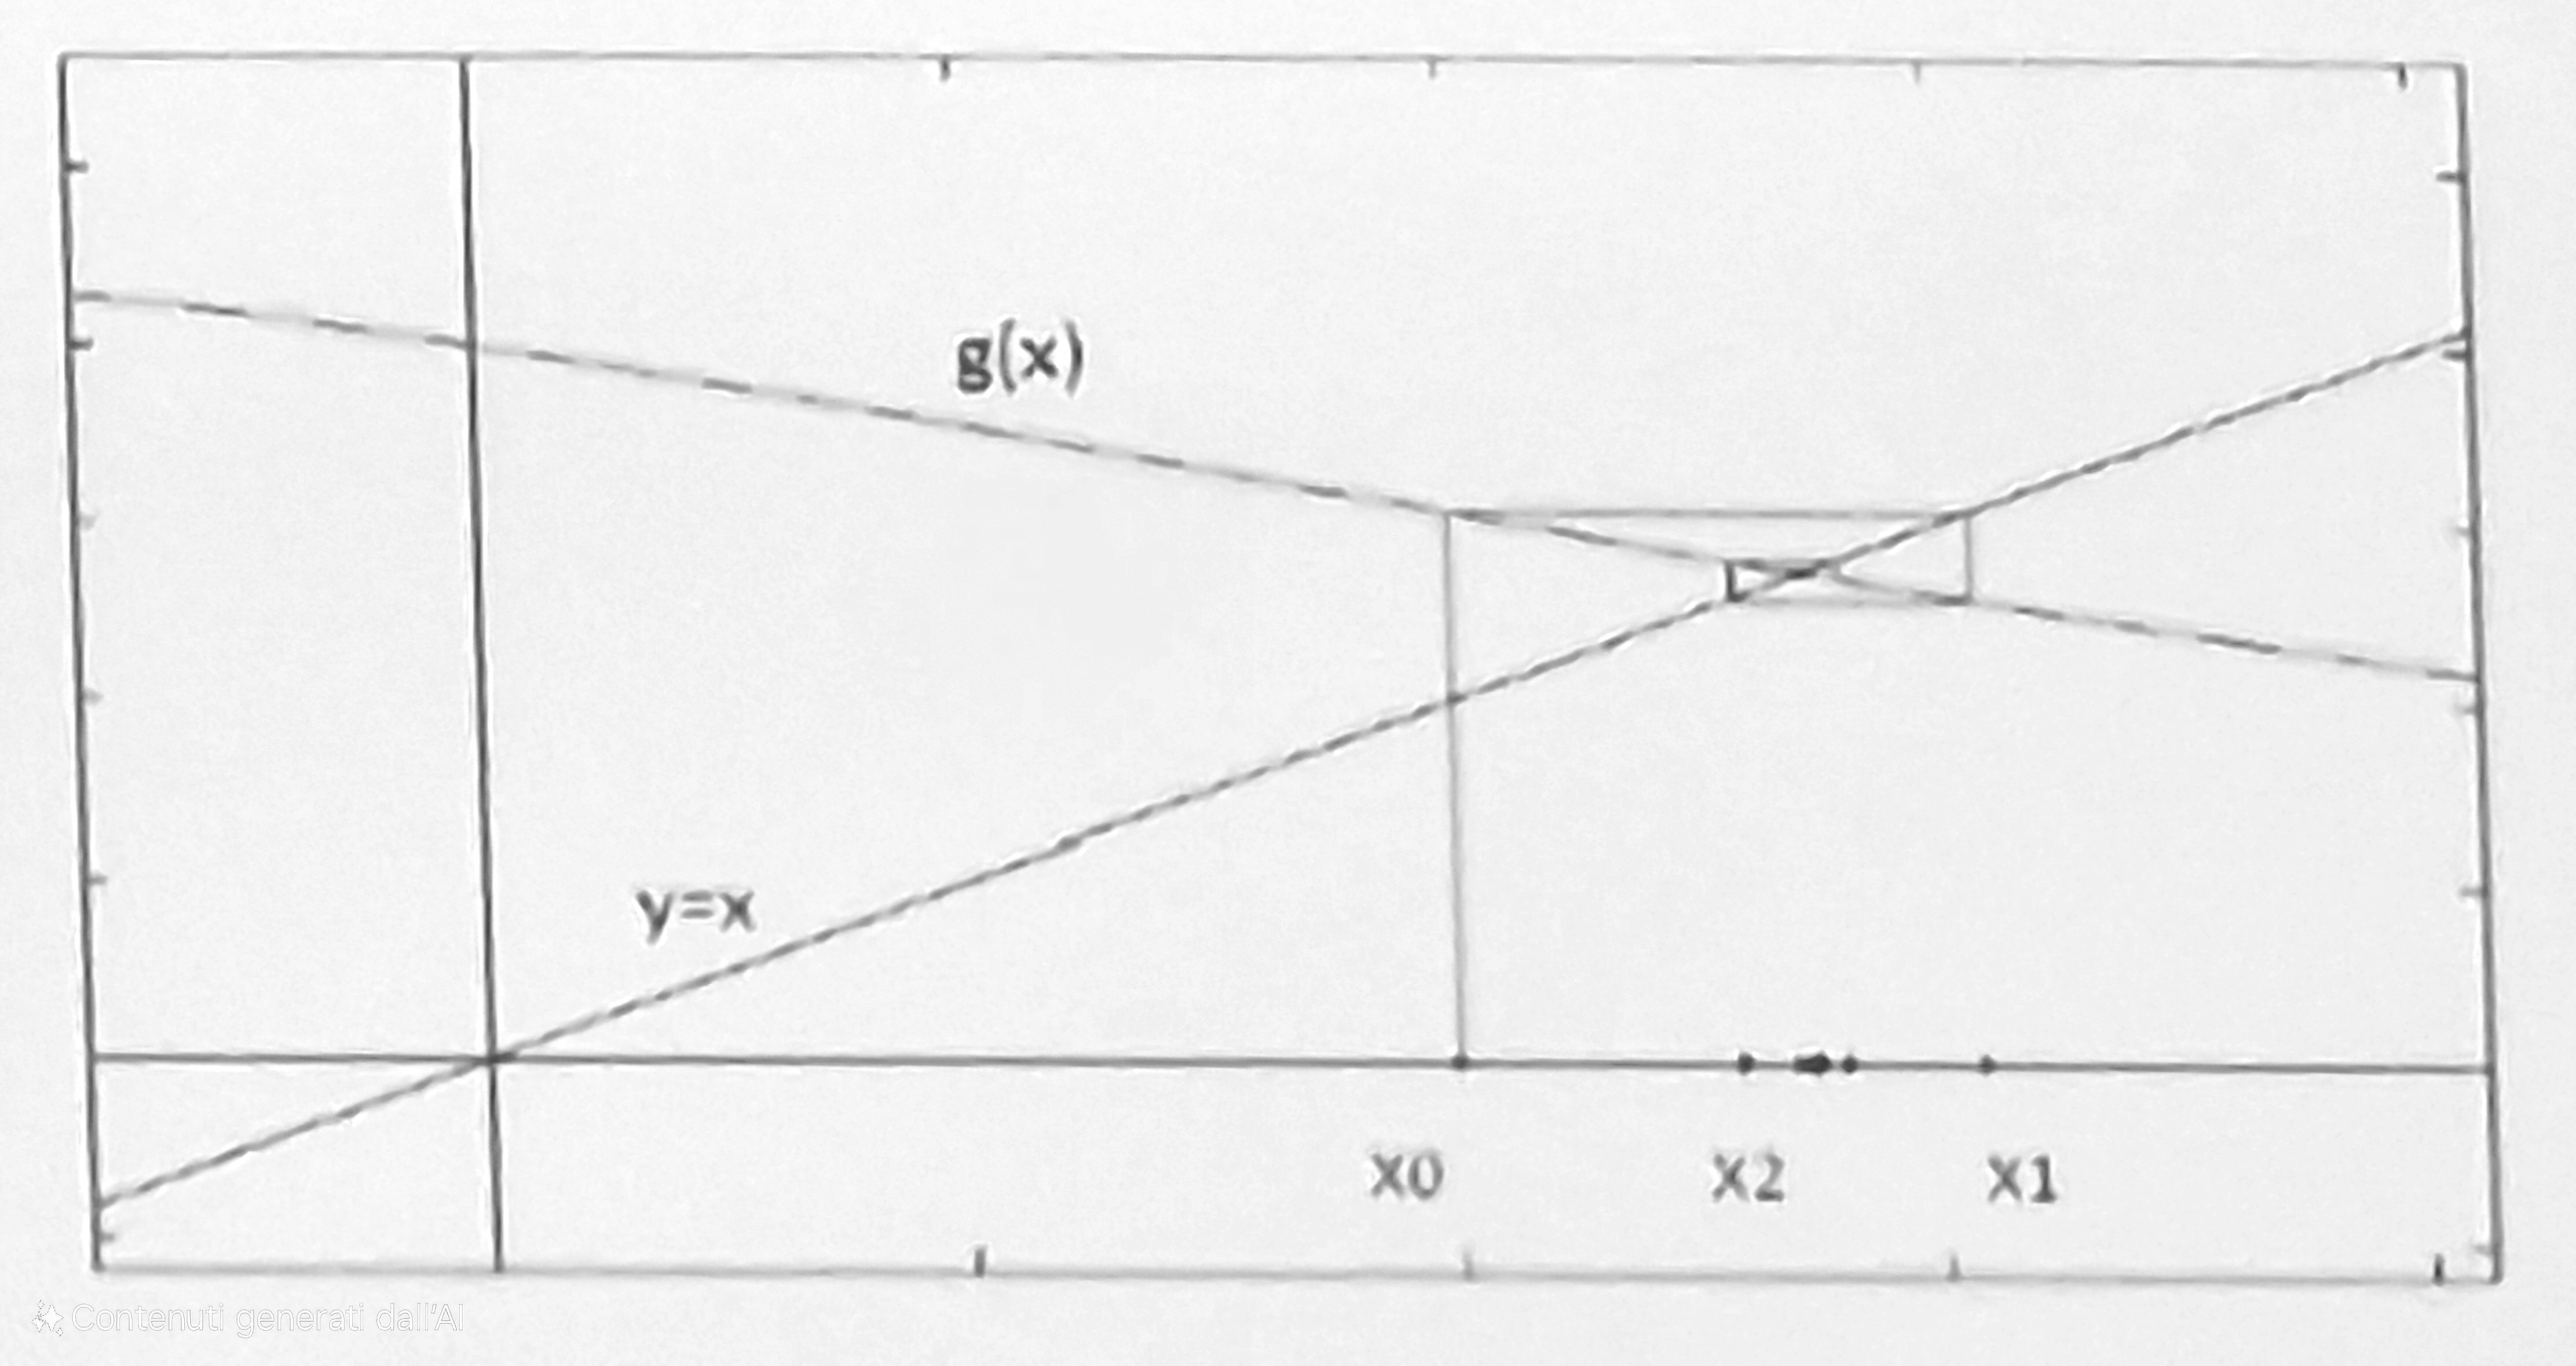
\includegraphics[width=1\textwidth]{Esterni/Altro/imgs/20250226_091358.jpg} 
    \caption{Grafico di andamento del sistema iterativo.} 
    \label{fig:grafico_andamento_sistema_iterativo} 
\end{figure}

\todo{commenti sul quaderno}
\begin{notion}
    La convergenza dipende dalla pendenza della curva ed è collegata alla definizione di contrattività.
\end{notion}
Per dire che la funzione $x$ è decrescente basta avere un coefficiente angolare negativo, in altre parole $g'(x) < 0$, tuttavia questo implicherebbe una pendenza forte, che noi non vogliamo altrimenti non è garantita la convergenza.
Questo implica che $|g'(x)|$ deve essere sufficientemente piccolo.
\todo{test grafico + pendente sul quad (controesempio)}
\newline
\begin{notion}
    Se la derivata $g'(x)$ è sempre negativa, a prescindere dalla non derivata $g(x)$, la successione diverge.
    \newline
    Viceversa, se la derivata $|g'(x)|$ è sufficientemente piccola \textbf{(ma non troppo)} la funzione converge.    
\end{notion}
\todo{grafico con funzione crescente (sul quaderno)}
\begin{definition}
    $\mathit{g}(x)$ è contrattiva se esiste $0 < \lambda < 1$ tale che:
    \begin{equation}
        |g(x')-g(x'')|\leq \lambda|(x' - x'')|, \qquad \forall x',x''.        
    \end{equation}
\end{definition}
\begin{theorem}
    Sia $\mathit{g}(x)\in \mathcal{C}^1[a,b]$ tale che $\mathit{g}(x) \in [a,b]$ per tutti gli $x \in [a,b]$
\end{theorem}
\todo{continuare dalla foto sul cell}

\newpage
\begin{ex}
    Calcolo dell'approssimazione della radice reale dell'equazione i Fibonacci:
    \begin{displaymath}
        x^3+2x^2+10x-20=0
    \end{displaymath}
    con le possibili funzioni di iterazioni:
    \begin{displaymath}
        g_1(x) = \frac{20}{x^2+2x+10}
    \end{displaymath}
    \begin{figure}[h!]
        \centering 
        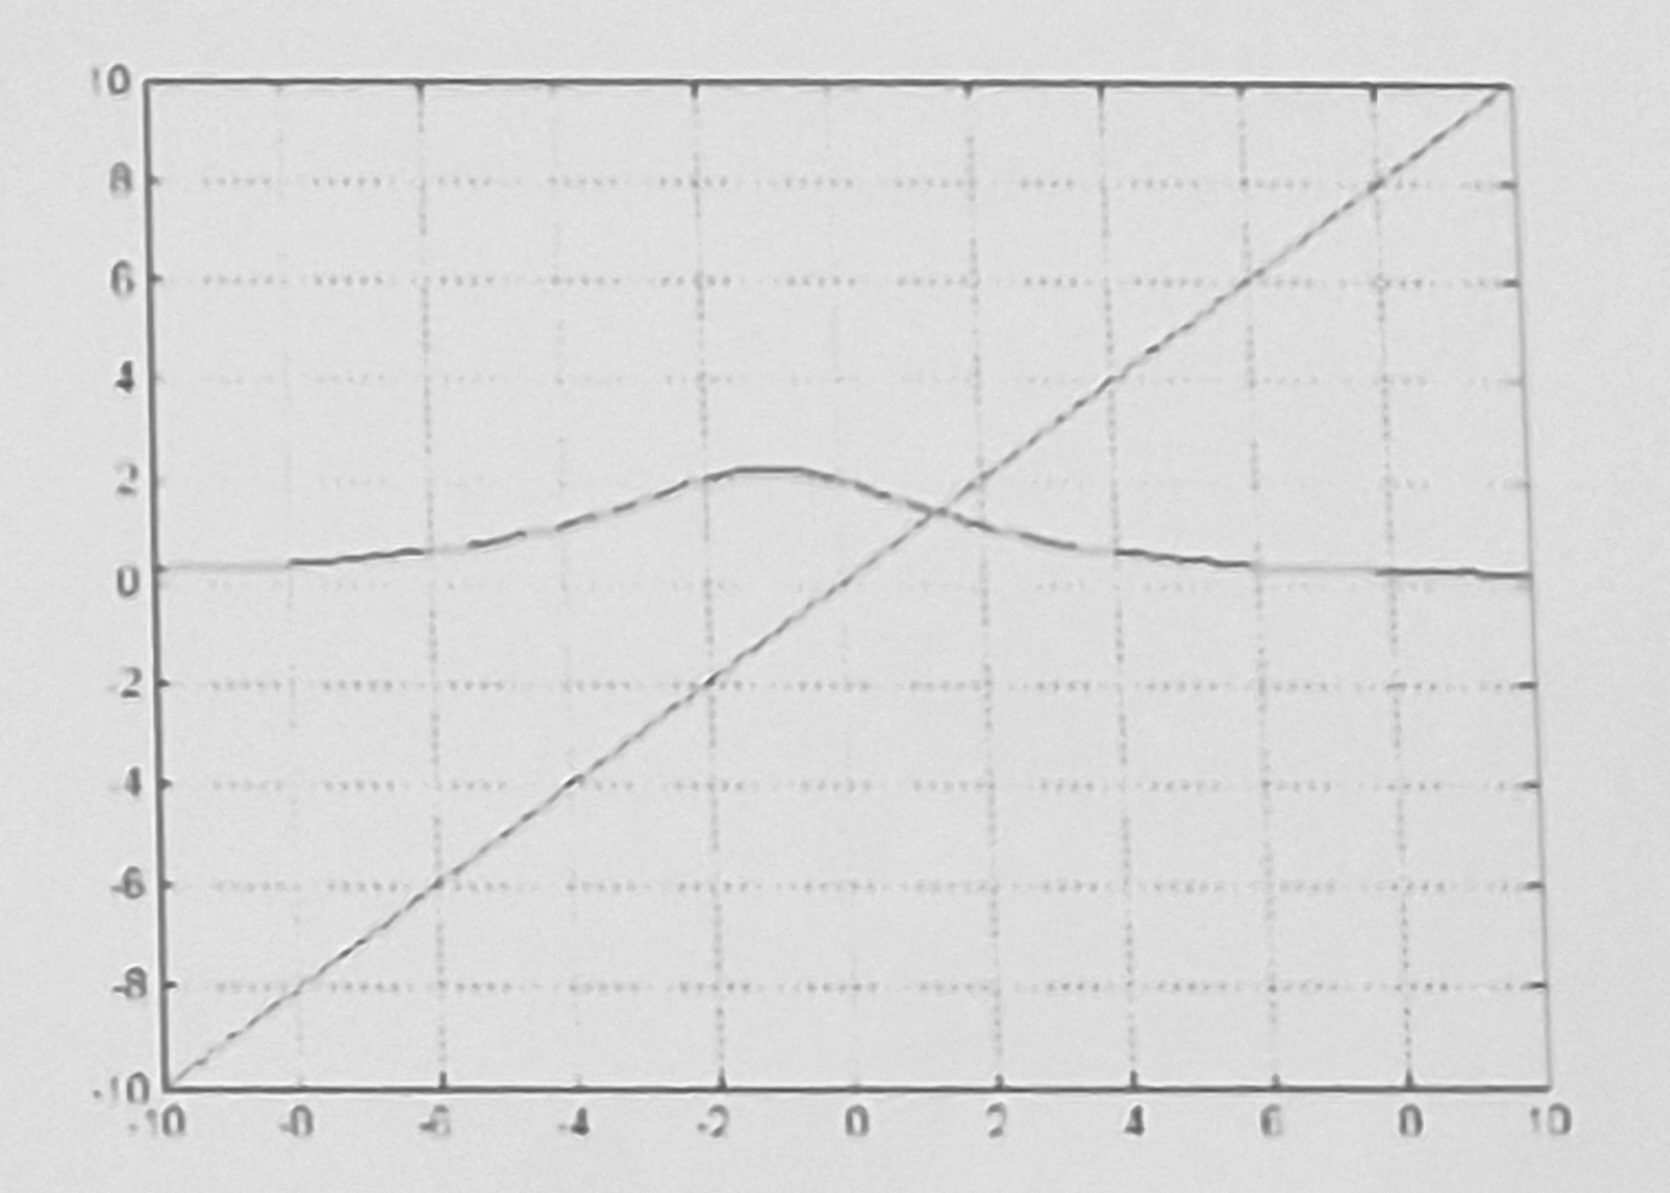
\includegraphics[width=0.5\textwidth]{Esterni/Altro/imgs/20250226_095026.jpg} 
        \caption{Grafico di iterazione Fib.1 (spirale mancante).} 
        \label{fig:fib1} 
    \end{figure}
\end{ex}
\begin{ex}
    Calcolo dell'approssimazione della radice reale dell'equazione i Fibonacci:
    \begin{displaymath}
        x^3+2x^2+10x-20=0
    \end{displaymath}
    con le possibili funzioni di iterazioni:
    \begin{displaymath}
        g_2(x) = \frac{20-10x}{x^2+2x}
    \end{displaymath}
    \begin{figure}[h!]
        \centering 
        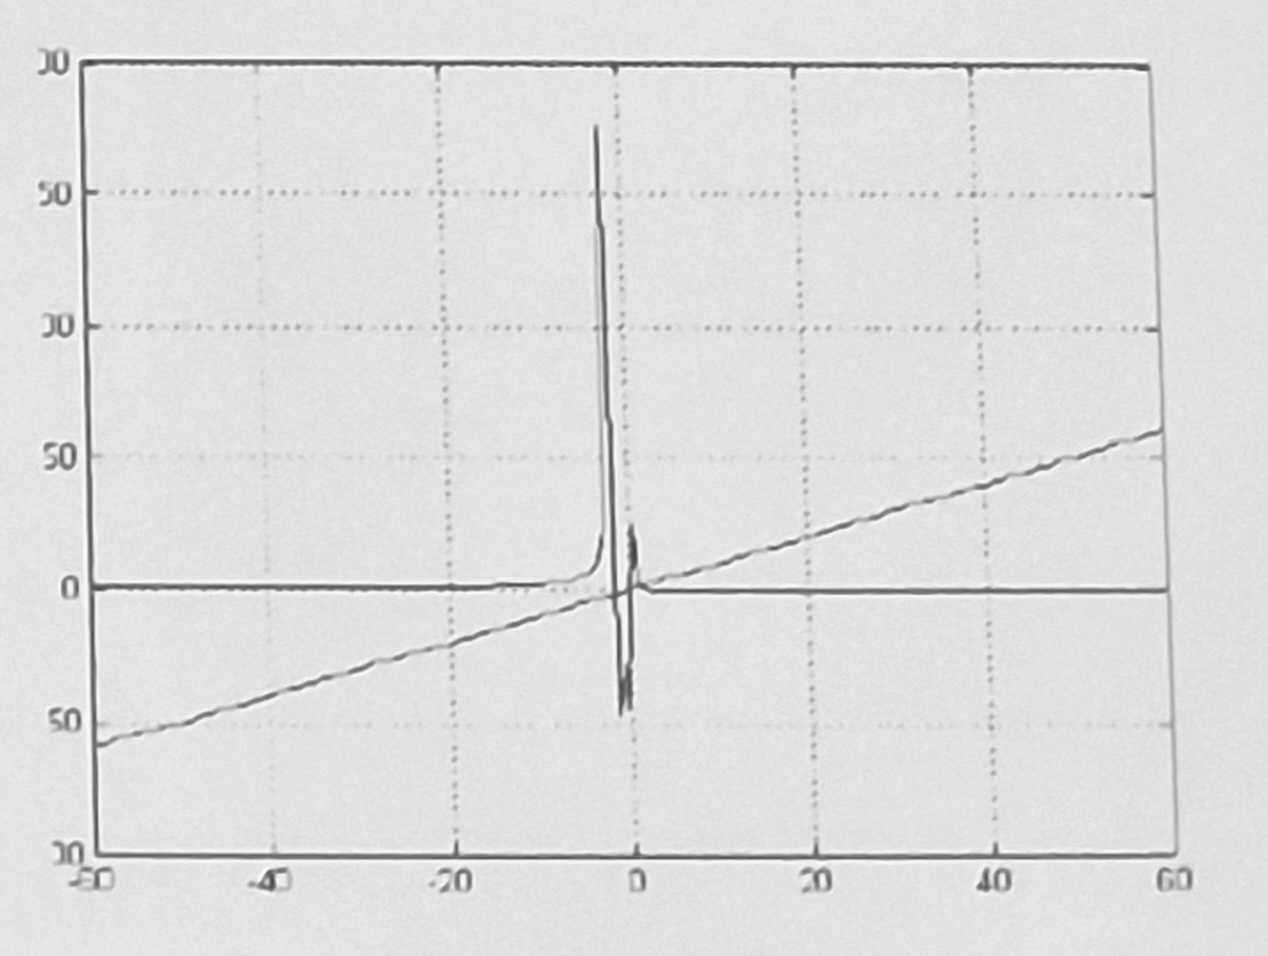
\includegraphics[width=0.5\textwidth]{Esterni/Altro/imgs/20250226_095154.jpg} 
        \caption{Grafico di iterazione Fib.2 (spirale mancante).} 
        \label{fig:fib2} 
    \end{figure}
\end{ex}

\newpage
\begin{figure}[h!]
    \centering 
    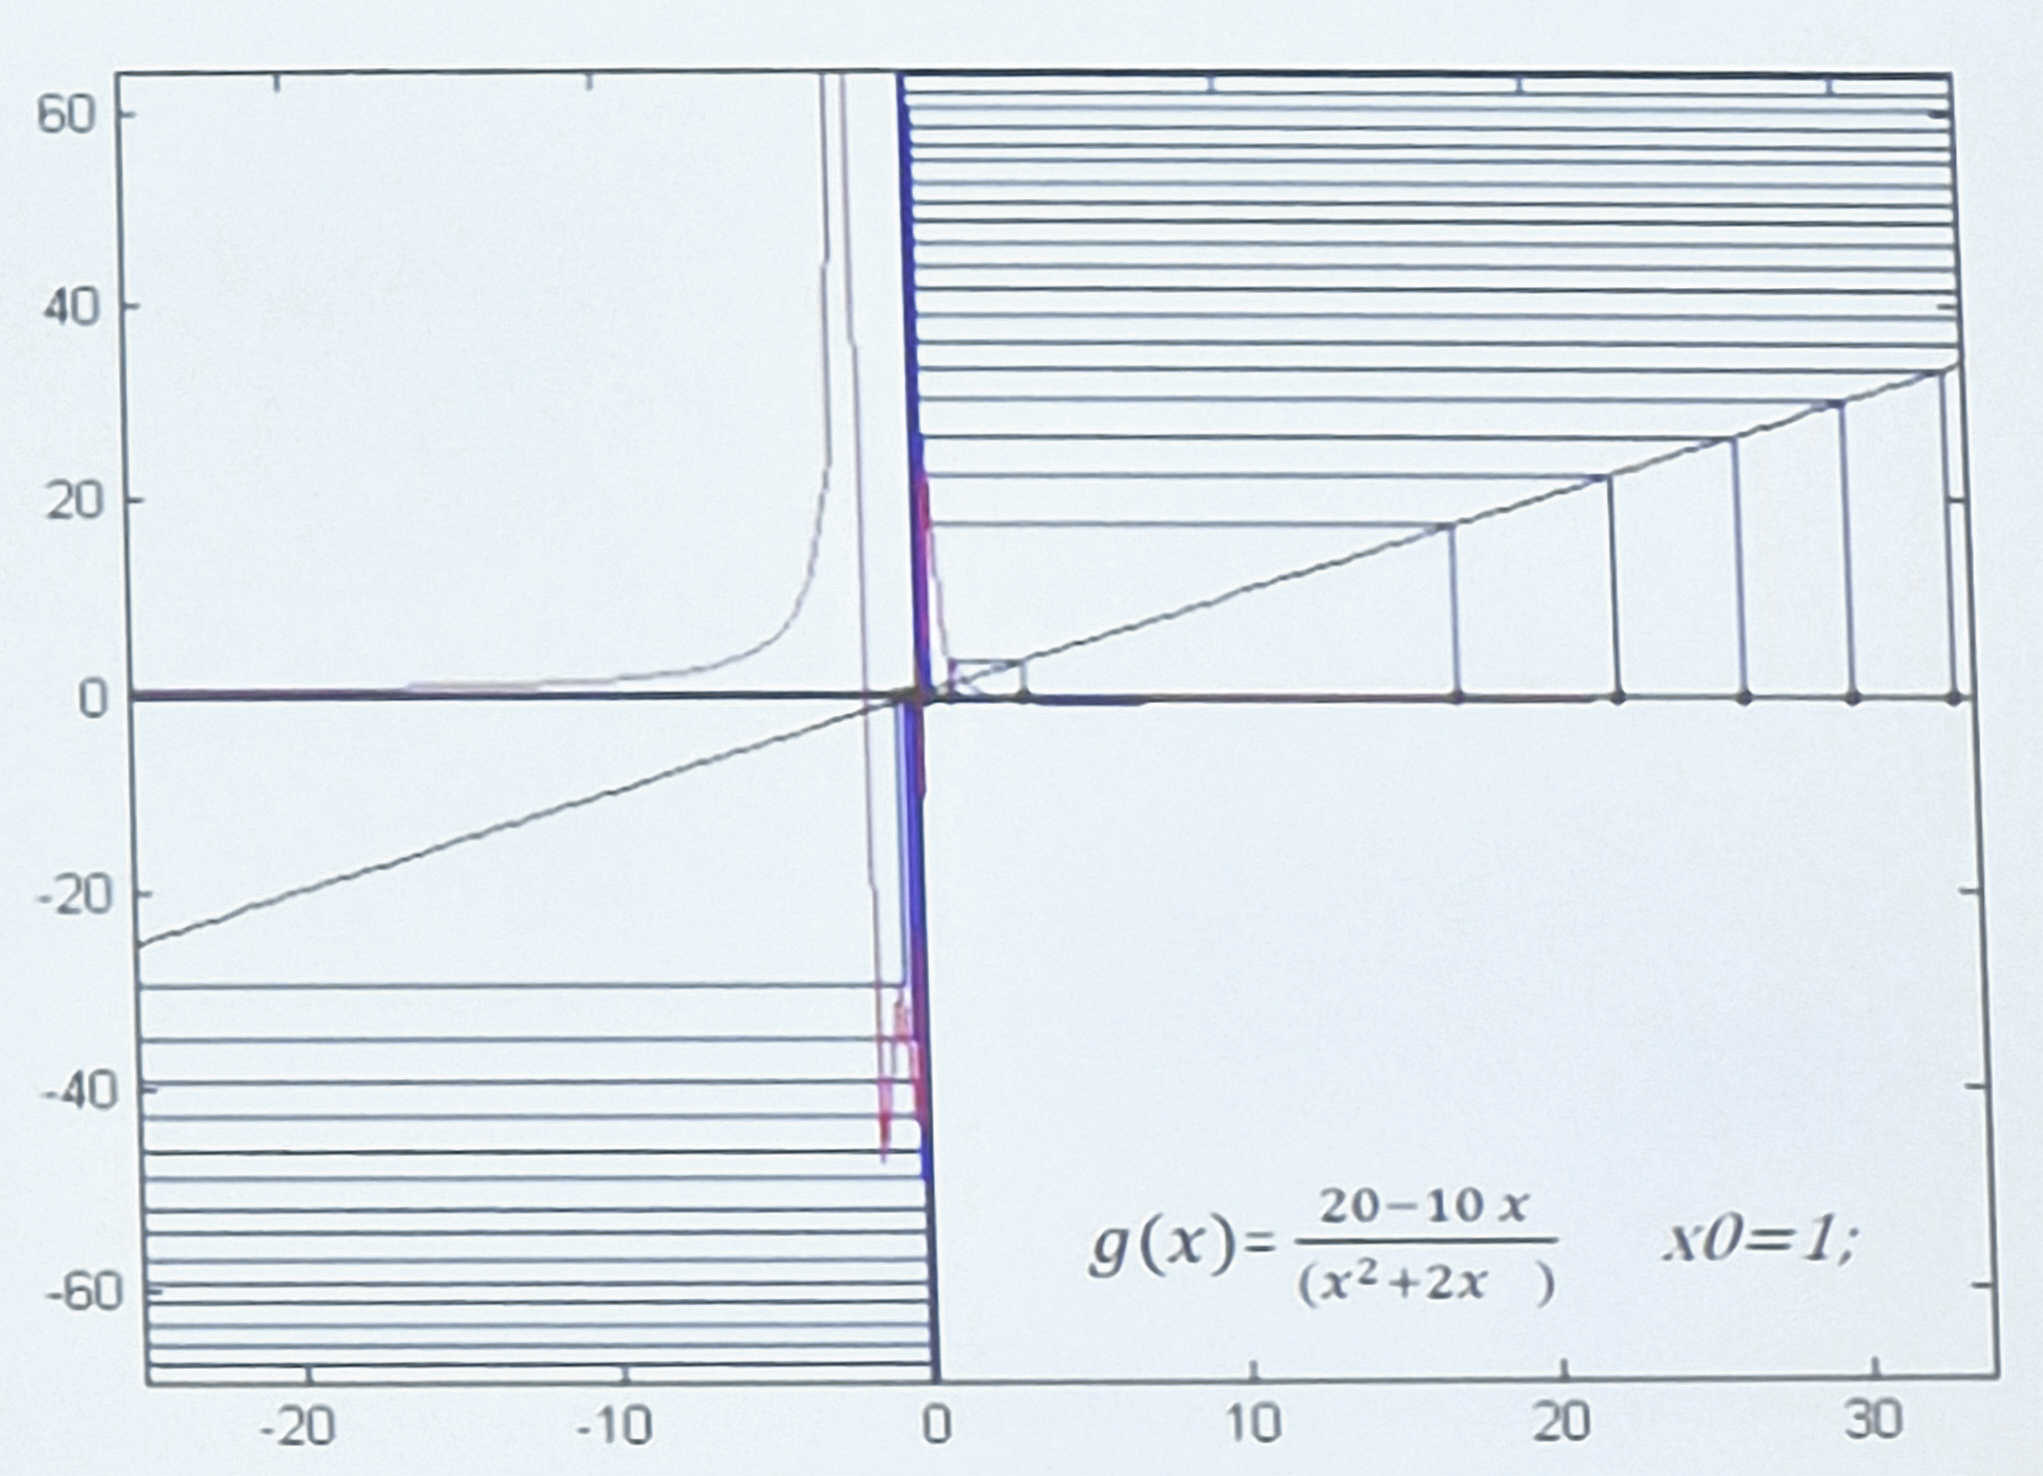
\includegraphics[width=0.6\textwidth]{Esterni/Altro/imgs/20250226_095648.jpg} 
    \caption{Esempio di divergenza.} 
    \label{fig:fib3} 
\end{figure}

\subsection{Metodi e processi iterativi}
Spesso, vengono prodotte simulazioni per analizzare ottimi locali e globali, ad esempio:
\begin{figure}[h!]
    \centering 
    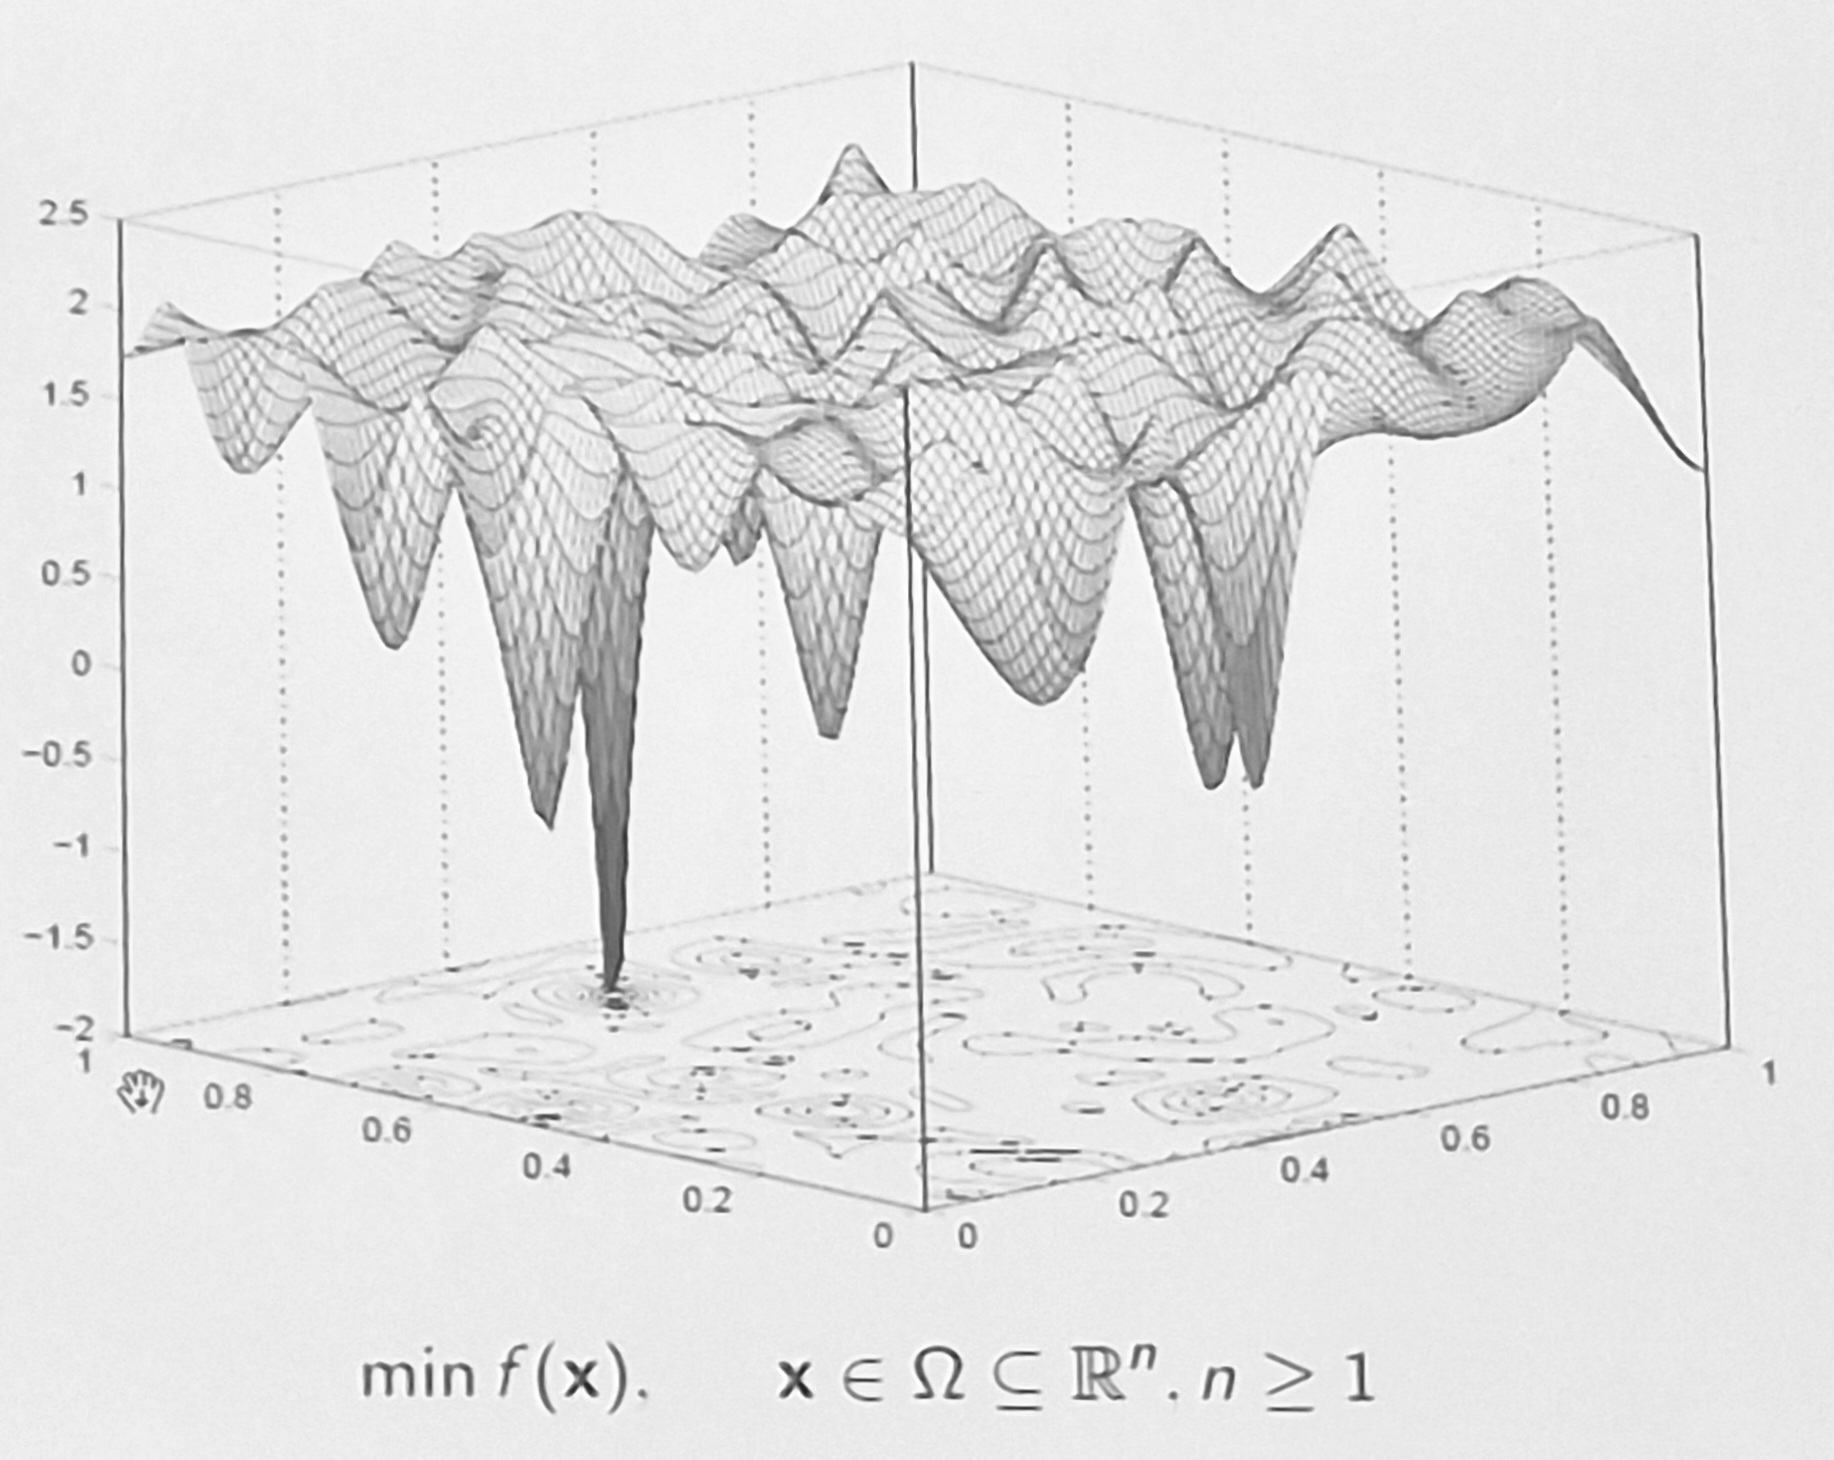
\includegraphics[width=0.8\textwidth]{Esterni/Altro/imgs/20250226_103050.jpg} 
    \caption{Ottimizzazione Globale.} 
    \label{fig:glob_ott} 
\end{figure}
tuttavia, per alcuni problemi ingegneristici non è sufficiente conoscere i massimi o minimi locali, bensì è importante studiare solo il caso peggiore o migliore (casi globali).
Un esempio di questo tipo potrebbe essere l'esempio per il carico strutturale di una struttura, dove basta semplicemente conoscere il carico massimo supportato (che corrisponde al caso peggiore: il crollo della struttura).

\newpage
\begin{equation}
    min(f(x)). \qquad x \in \Omega \subseteq \mathbb{R}^n. \qquad n\geq 1
\end{equation}
La funzione $f:\Omega \rightarrow \mathbb{R}$ è detta funzione obiettivo. $\Omega$ è un vettore che viene costruito a partire da un insieme semplice, come il rettagono generalizzato in fig[1.5]; 
L'insieme $\Omega \subseteq \mathbb{R}^n$ è detto insieme (o regione) ammissibile:
\begin{displaymath}
    \Omega=\{x=(x_1,x_2, \cdots, x_n)\in D \subseteq \mathbb{R}^n: g_j(x)\leq 0. \qquad j = 1, 2, \cdots, m\};
    D = \{x=(x_1,x_2, \cdots, x_n)\in \mathbb{R}^n:a_i<b_i\cdot a_i < b_i.a_i < b_i. \qquad i = 1, 2, \cdots, n\}.
\end{displaymath}
Vengono studiati esistenza ed unicità della soluzione, tramite il teorema di Weiestrass\myfootnote{
        Se la funzione è continua in un intervallo (o regione) chiuso e limitato, la funzione raggiungerà dei punti massimi e minimi.
    }.

\begin{figure}[h!]
    \centering 
    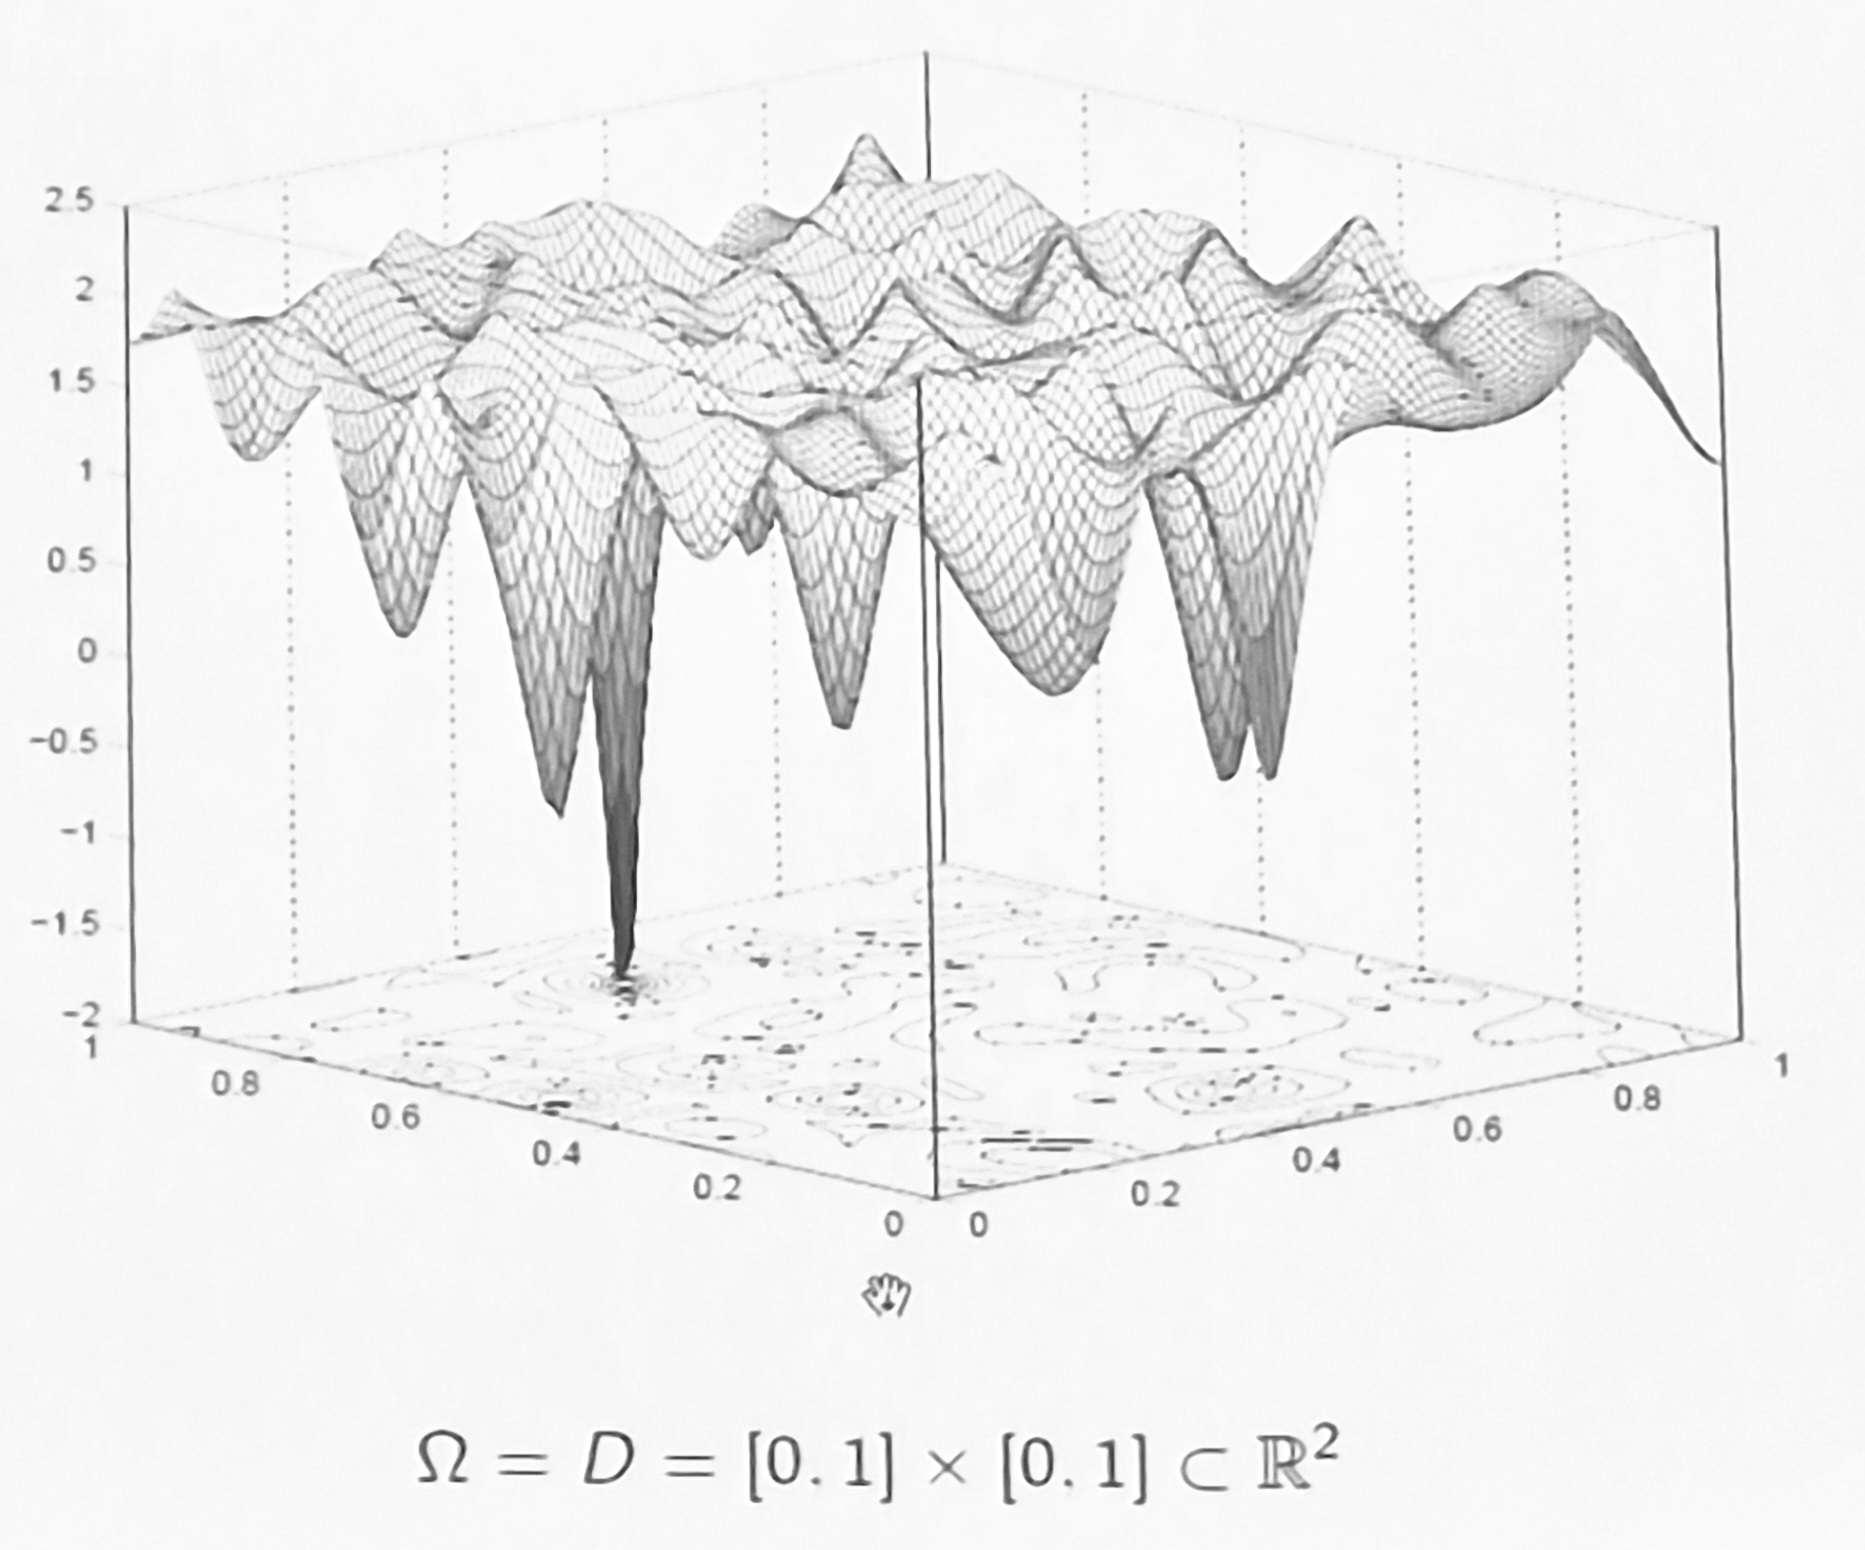
\includegraphics[width=0.8\textwidth]{Esterni/Altro/imgs/20250226_104634.jpg} 
    \caption{Regione ammissibile del caso in analisi.} 
    \label{fig:glob_ott_amm_reg} 
\end{figure}

\newpage
\todo{def. min e max globale sul cell}
Se siamo in possesso di una funzione che produce come output il minimo di una funzione, negando la funzione e cambiando di segno l'output, otterremo in output il massimo della funzione.
\begin{figure}[h!]
    \centering 
    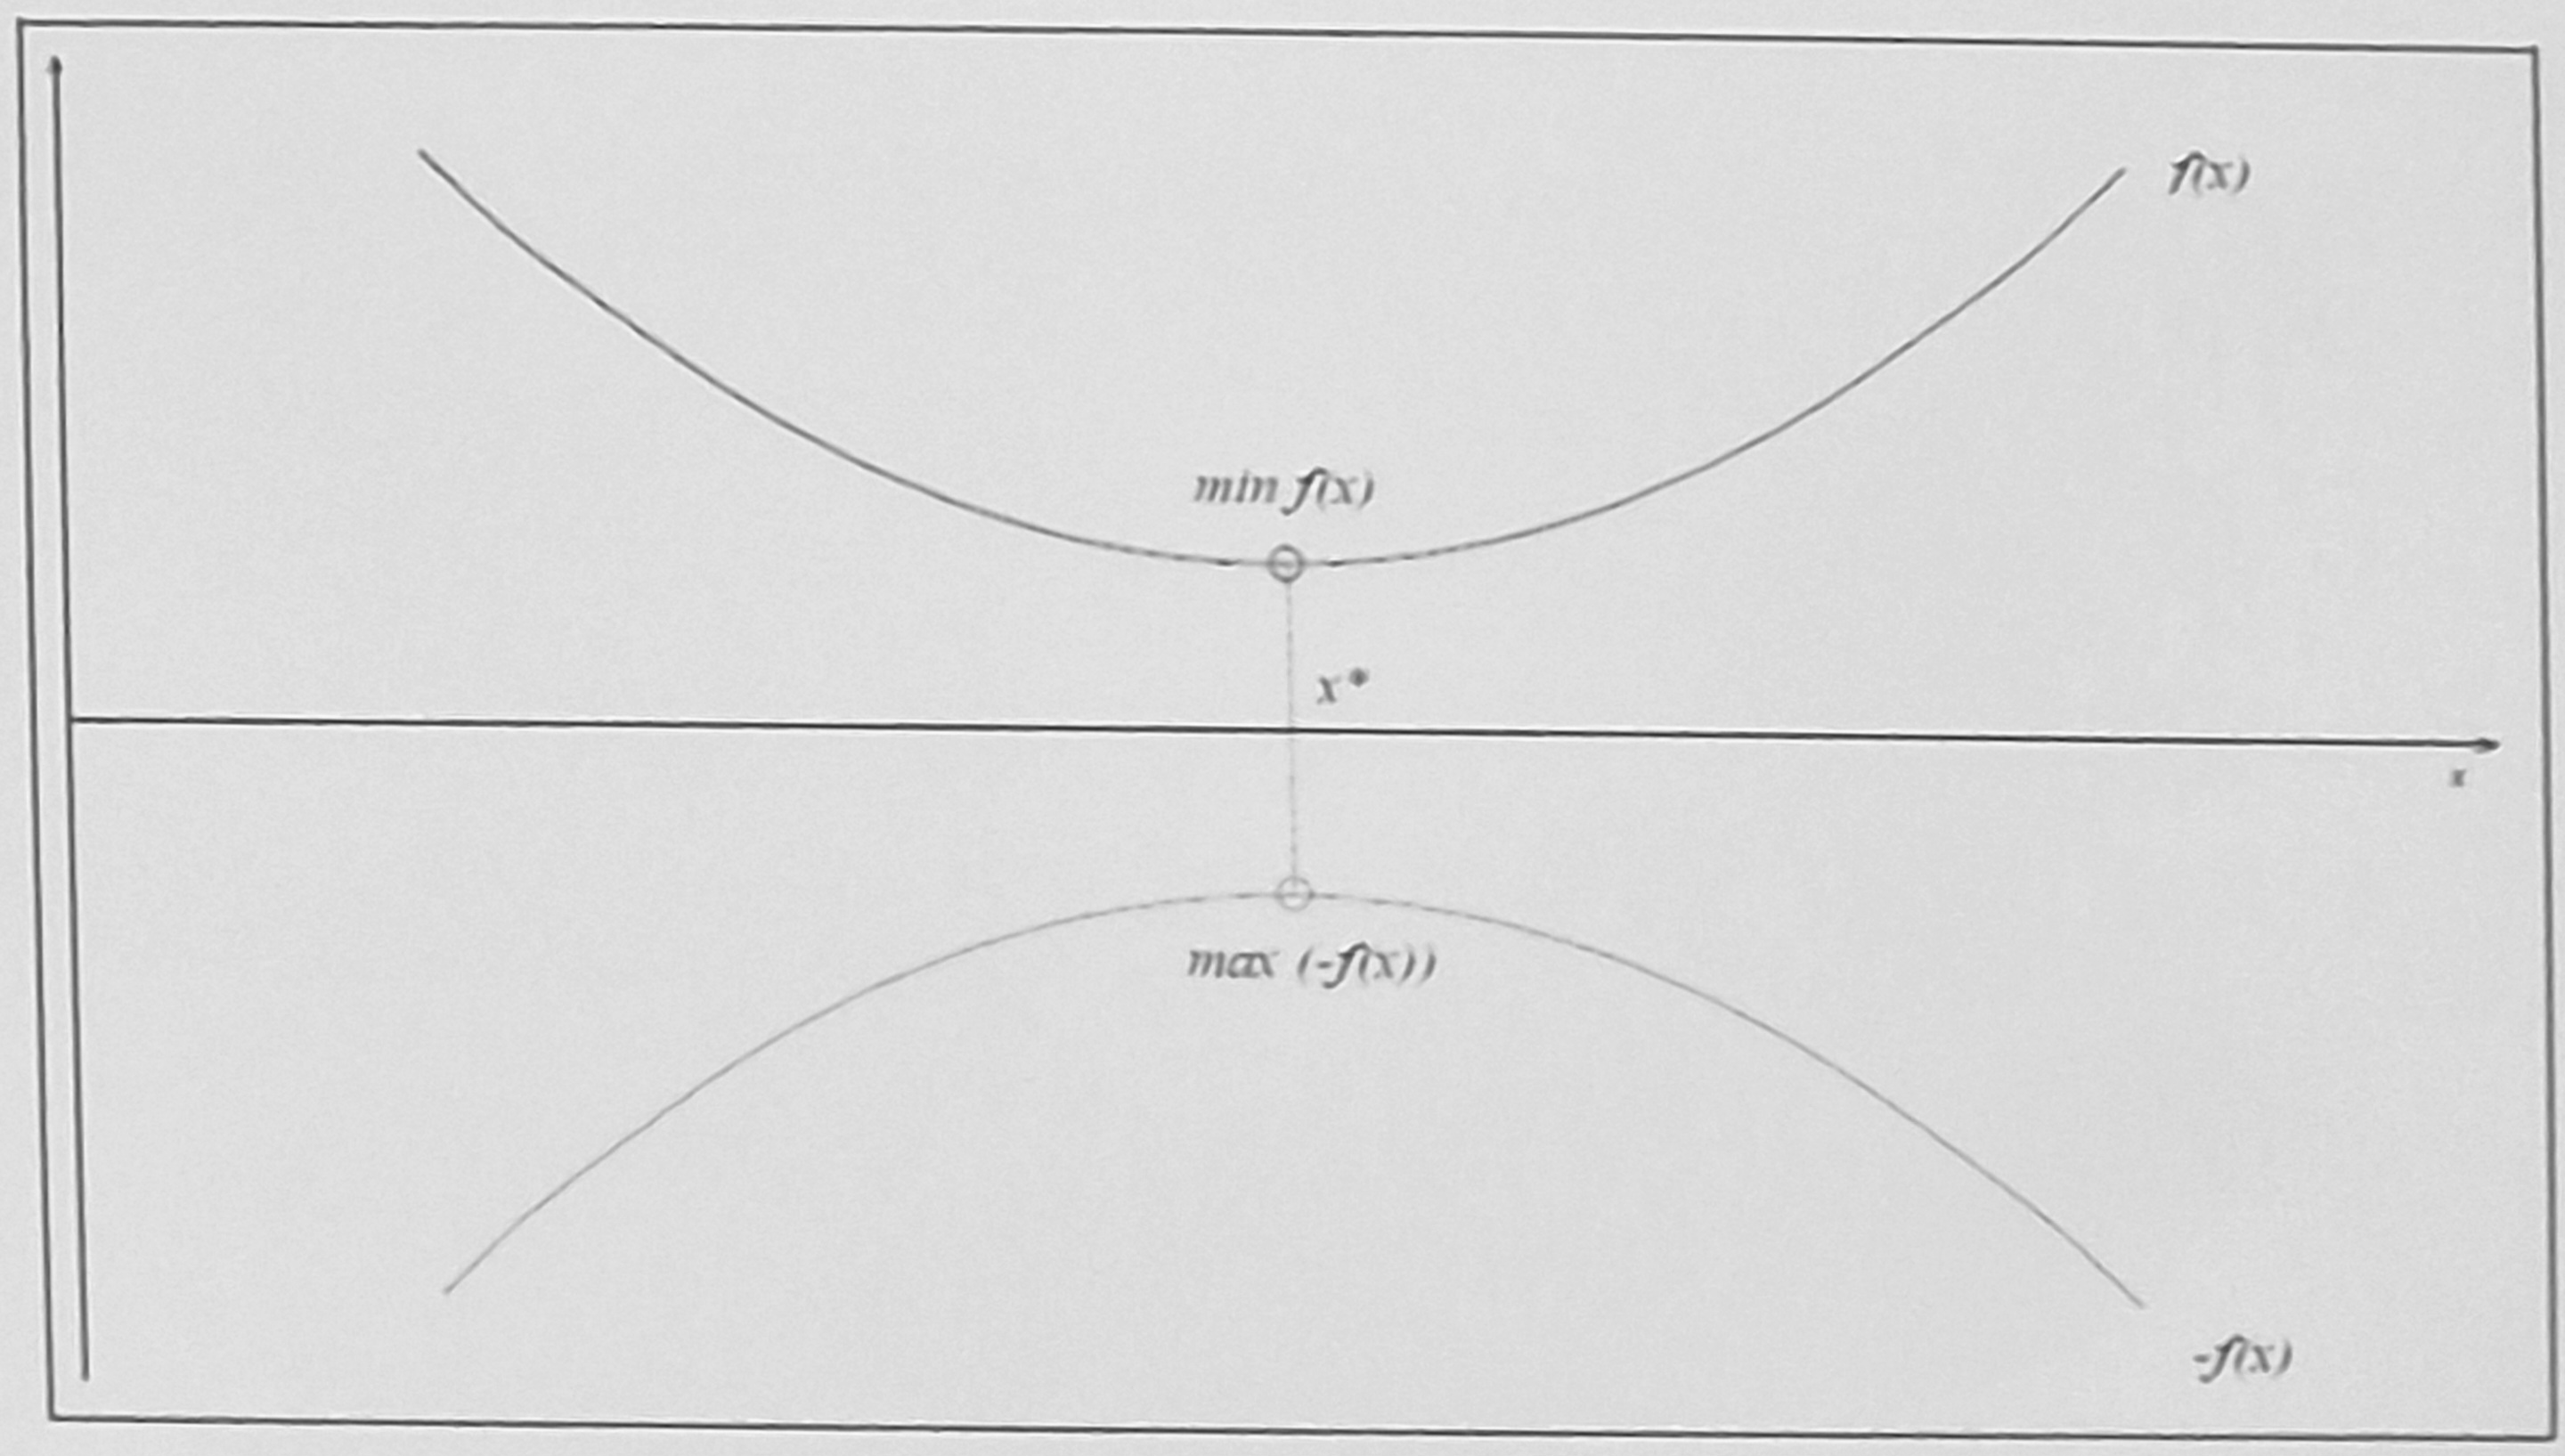
\includegraphics[width=0.8\textwidth]{Esterni/Altro/imgs/20250226_105033.jpg} 
    \caption{Regione ammissibile del caso in analisi.} 
    \label{fig:glob_ott_amm_reg} 
\end{figure}

\subsubsection{Problema di ottimizzazione globale}
Il problema in analisi è il seguente:
\begin{displaymath}
    f^* = f(x^*) = \min_{x \in [a, b]}f(x)
\end{displaymath}
La soluzione esiste (Teorema di Weiestrass) e supponiamo sia unica.
\begin{figure}[h!]
    \centering 
    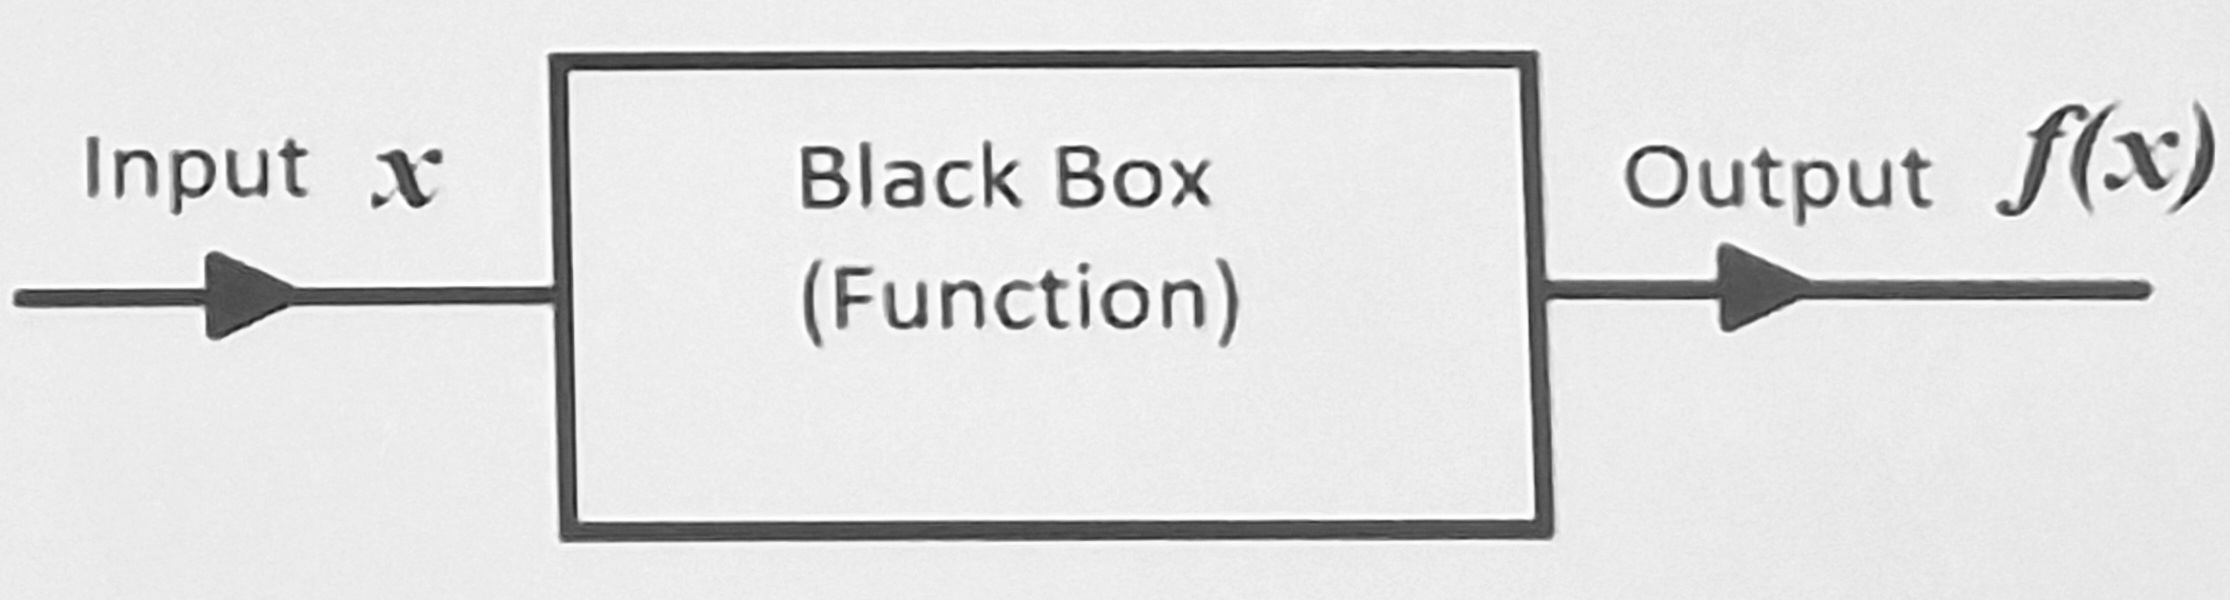
\includegraphics[width=0.8\textwidth]{Esterni/Altro/imgs/20250226_105447.jpg} 
    \caption{Regione ammissibile del caso in analisi.} 
    \label{fig:glob_ott_amm_reg} 
\end{figure}
Solitamente la funzione viene data a scatola nera, spesso perché non esiste una vera e propria forma finita per descriverla, sappiamo solo che è continua.
\newline
Non essendo in possesso della formula analitica sarà impossibile utilizzare tecniche come derivate o minimi locali.

\newpage
Così si assume che la funzione vine data da un simulatore, poiché il costo computazionale è elevato a causa della sua rappresentazione analitica.
La valutazione è costosa, per ragioni temporali o addirittura per prove fisiche, ergo sperimentazioni che comportano l'utilizzo di macchine.
\newline 
Seppur non conoscendo la funzione è possibile conoscere la famiglia della stessa funzione:
\newline
\textbf{Univotale:}
\begin{figure}[h!]
    \centering 
    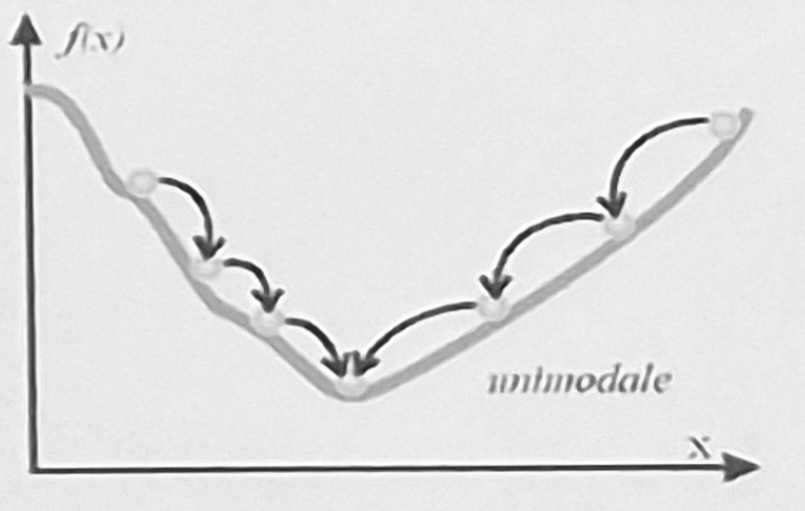
\includegraphics[width=0.6\textwidth]{Esterni/Altro/imgs/t1.jpg} 
    \caption{Funzione "univotale", possiede solo un minimo (questa è anche convessa).} 
    \label{fig:type1} 
\end{figure}
\\
\textbf{Multiestremale:}
\begin{figure}[h!]
    \centering 
    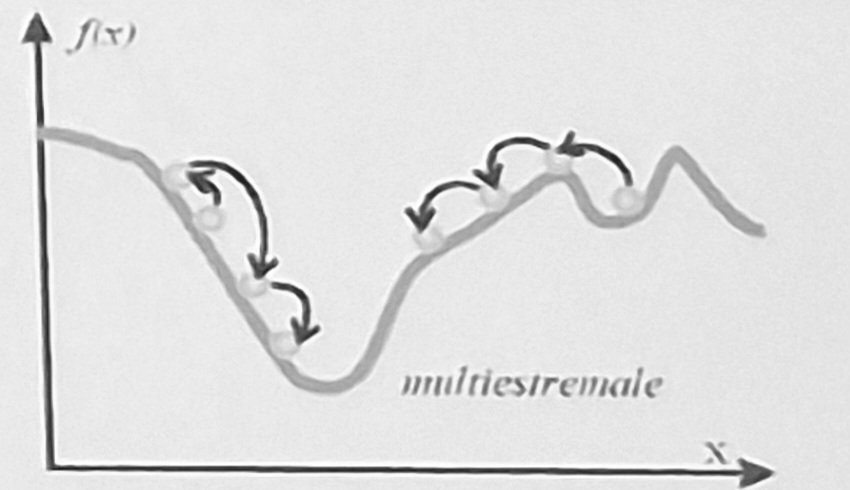
\includegraphics[width=0.6\textwidth]{Esterni/Altro/imgs/t2.jpg} 
    \caption{Funzione "multiestremale", possiede più minimi e/o massimi locali.} 
    \label{fig:type2} 
\end{figure}

\newpage
\begin{figure}[h!]
    \centering 
    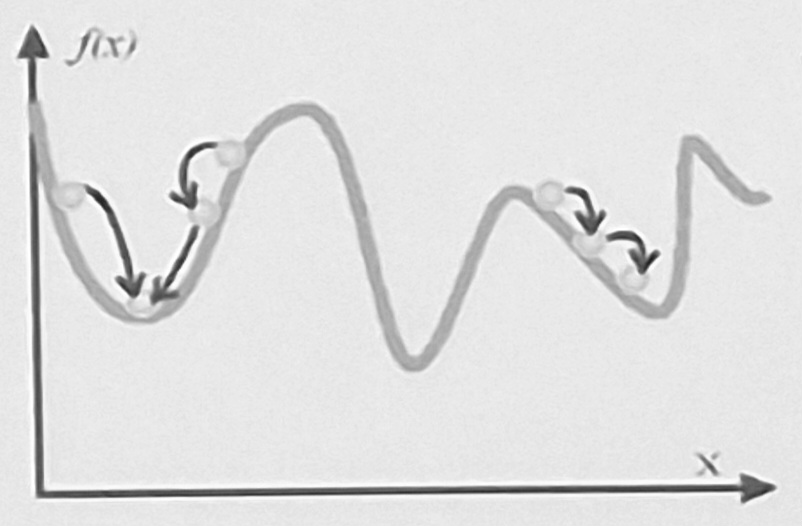
\includegraphics[width=0.6\textwidth]{Esterni/Altro/imgs/t3.jpg} 
    \caption{ Funzione "multivotale" ben condizionata, piccole perturbazioni non implicano grandi variazioni.} 
    \label{fig:type3} 
\end{figure}
\begin{figure}[h!]
    \centering 
    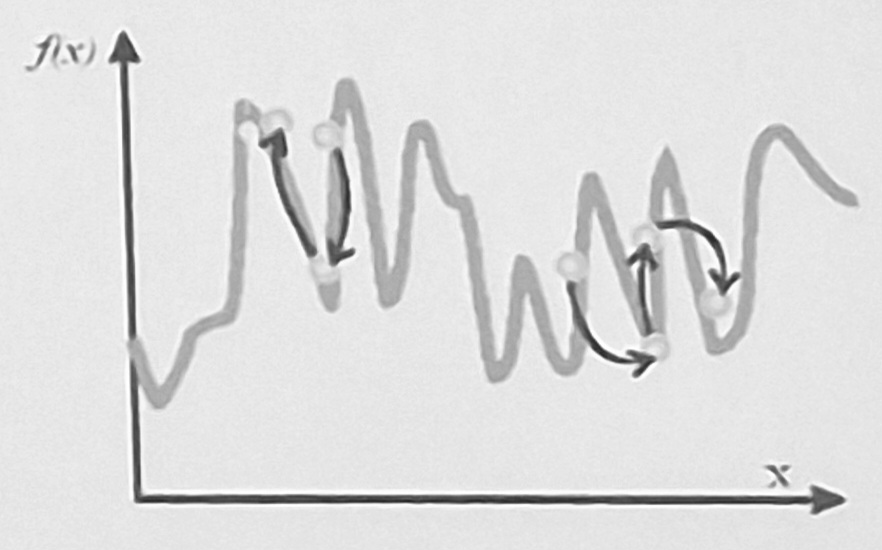
\includegraphics[width=0.6\textwidth]{Esterni/Altro/imgs/t4.jpg} 
    \caption{ Funzione "multivotale" mal condizionata, piccole perturbazioni implicano grandi variazioni.} 
    \label{fig:type4} 
\end{figure}
\begin{figure}[h!]
    \centering 
    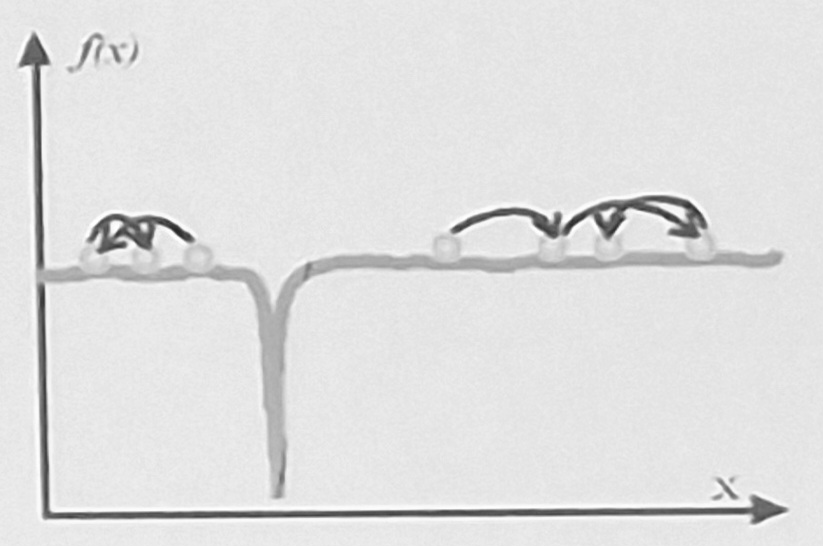
\includegraphics[width=0.6\textwidth]{Esterni/Altro/imgs/t5.jpg} 
    \caption{ Funzione "multivotale" mal condizionata e costante (gravissimo), non ho possibilità di dare garanzie.} 
    \label{fig:type5} 
\end{figure}
\newpage
\begin{figure}[h!]
    \centering 
    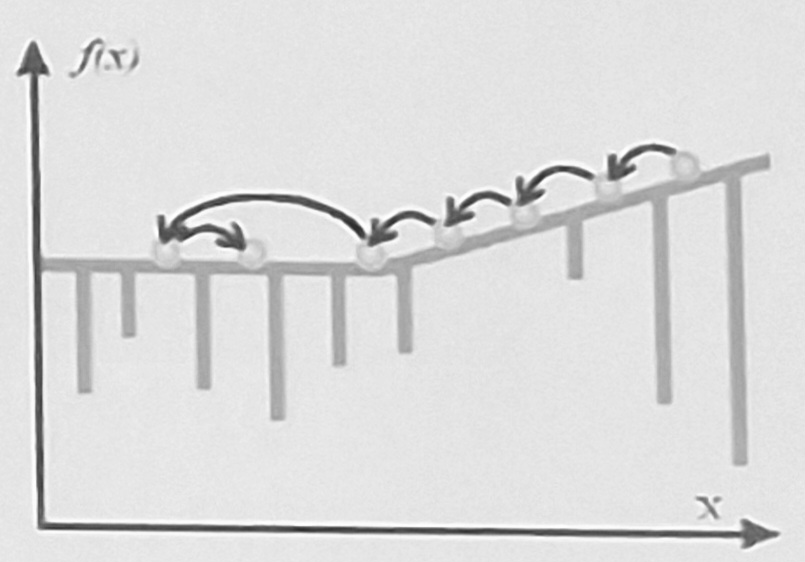
\includegraphics[width=0.6\textwidth]{Esterni/Altro/imgs/t6.jpg} 
    \caption{ Funzione "multivotale" mal condizionata a tal punto da essere inaccettabile poiché presenta punti infinitesimali indistinguibili.} 
    \label{fig:type6} 
\end{figure}

\newpage
\begin{notion}
    Si può evincere dalla continuità delle sei funzioni presentate che, \textbf{la continuità della funzione non garantisce la bontà della soluzione}.
\end{notion}
\chapter{Analisi degli errori numerici
}
\chapter{Capitolo}
\chapter{Capitolo}
\chapter{Capitolo}
\chapter{Capitolo}
\chapter{Esercitazioni}
\textbf{Contatto: } francesco.toscarella@unical.it
\newline
\section{Esercitazione 1}
\subsubsection{MATLAB}
MATLAB\myfootnote{
    MATrix LABoratory (non Mathematical Laboratory).
} è un software di calcolo. Una sua caratteristica è quella di vedere ogni tipo di input come una matrice, per intenderci, uno scalare in MATLAB è una matrice $1\times 1$.
MATLAB è a pagamento, tuttavia, esistono molte alternative come "Scilab" o "Octab" che invece sono gratuite\myfootnote{
    Sul web è possibile trovare anche traduttori da MATLAB a Scilab.
}.
\subsubsection{Sintassi}
MATLAB è case sensitive.
\begin{itemize}
    \item a = 1 $\rightarrow$ istanzia la variabile e ne stampa subito il risultato.
    \item b = 1; $\rightarrow$ istanzia la variabile e non stampa il risultato.
    \item ans $\rightarrow$ è una variabile temporanea che prende il valore risultato da un operazione che abbiamo eseguito.
    \item clear $\rightarrow$ pulisce tutto il workspace.
    \newpage
    \item vector = {1 2 3} oppure {1,2,3} $\rightarrow$ definisce un vettore riga vector.
    \item vector = {1; 2; 3} $\rightarrow$ definisce un vettore colonna vector.
    \item matrix = matrice $\rightarrow$ definisce una matrice matrix.
    \item +,-,/,* $\rightarrow$ operazioni aritmetiche.
    \item length(x) $\rightarrow$ restituisce la dimensione maggiore della matrice, ad esempio vettore riga $1\times 4$ restituisce $4$, un vettore colonna $5\times 1$ restituisce $5$.
    \item $mat\_a \quad .* \quad mat\_b;$ $\rightarrow$ prodotto tra due matrici, \textbf{elemento per elemento}.
    \item $mat\_a \quad * \quad mat\_b;$ $\rightarrow$ prodotto matriciale, \textbf{riga per colonna}.
    \item $mat\_a \quad ./ \quad mat\_b;$ $\rightarrow$ divisione tra due matrici, \textbf{elemento fratto elemento}.
    \item $mat\_a \quad / \quad mat\_b;$ $\rightarrow$ divisione matriciale, \textbf{riga fratto colonna}.
    \item a = ciao $\rightarrow$ verrà visto come una matrice $1 \times 4$
    \item strcat(x,y) $\rightarrow$ concatena due stringhe.
    \item abs(x) $\rightarrow$ valore assoluto.
    \item log(x) $\rightarrow$ logaritmo naturale.
    \item log10(x) $\rightarrow$ logaritmo in base 10.
    \item sqrt(x) $\rightarrow$ radice quadrata.
    \item exp(x) $\rightarrow$ esponenziale: $e^x$.
    \item zeros(n, m) $\rightarrow$ matrice di zeri di dimensione $n_righe \times m_colonne$.
    \item ones(n, m) $\rightarrow$ matrice di uno di dimensione $n_righe \times m_colonne$.
    \item zeros($n_1,n_2, \cdots, n_k$) oppure ones($n_1,n_2, \cdots, n_k$) $\rightarrow$ è possibile mettere quante dimensioni si vogliono.
    \item eye(n, m) $\rightarrow$ matrice identità di dimensione $n_righe \times m_colonne$.
    \item format long/short $\rightarrow$ mostra più o meno cifre significative.
    \newpage
    \item if condition
        \newline
        a = 1;
        \newline
        elseif condition
        \newline
        a = 2;
        \newline
        else
        \newline
        a = 3; $\rightarrow$ condizioni if, elseif, else.
    \item for i = 1:passo:x
        \newline
        ...codice...
        \newline
        end $\rightarrow$ ciclo for da 1 a x. NB: I vettori in MATLAB vanno da 1 in poi, il for può andare da $-\infty$ a $+\infty$, ma i vettori no.   
    \item while condition:
        \newline
        ...codice...
        \newline
        end $\rightarrow$ ciclo while.
\end{itemize} 

\printbibliography

%ringraziamenti

\end{document}